\begin{frame}[t]{C\'omo usar el software?}\vspace{10pt}

Cuando desees usar datos experimentales que \textit{no} est\'en en la base de datos:

\begin{enumerate}
	\item Pega la matriz experimental de variables dependientes e independientes en un archivo de texto. Procura que cada columna est\'e separada por una indentaci\'on TAB (normalmente, copiar y pegar directamente de Excel realiza esta acci\'on de manera autom\'atica).
	\item Guarda el archivo de texto en: App/DataBase/Datos
	\begin{figure}
		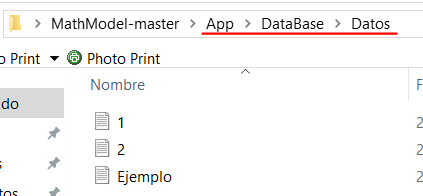
\includegraphics[scale=0.7]{Images/db.png}
	\end{figure}
\end{enumerate}

\vspace{0.5cm}

NOTA: La ejecuci\'on de cada comando, o bloque de programaci\'on dentro del notebook, es con CTRL + ENTER.

\end{frame}